\section{Algorithm Overview}
	Our A* waypoint system began with several guidelines and constraints around which to model a genetic algorithm. These guidelines would dictate the type of graph we wished to achieve from running our genetic algorithm. Having understood A* search itself, an ideal waypoint graph should only contain the \textbf{minimum number of nodes} required to quickly and efficiently traverse the maze through the search. Secondly, the graph should aim to achieve \textbf{full connectivity} of the maze's walkable space, meaning that any random point placed in the maze should be walkable to any other point in the maze by running A* search using the generated graph.
	
	With the attributes of an ideal A* waypoint graph in mind, we next considered the construction of a genetic algorithm to handle the evolution sequence for generating such a graph.
	
	\subsection{Initial Population}
	The initial starting population contained a set of \(x\) graphs, each of which would be generated using \(y\) randomly placed nodes in the walkable space of the graph. Each node in this set would be connected to every other node where line of sight visibility was present. Line of sight, for the purpose of this algorithm, was handled by Unity Engine's raycasting system. This means that for any given nodes \(a\) and \(b\) in the graph, such that \(a \neq b\), if a ray could be cast from \(a\) to \(b\) without intersecting with any wall of the maze, then \(a\) and \(b\) should be connected. This resulted in a fully connected graph along all walkable edges in the graph.
	
	\subsection{Evaluation}
	After the initial generation has been built, the genetic algorithm must then handle evaluating each graph, evaluating fitness for use later in the selection and crossover stages. Three immediate factors were used to score graphs in this implementation. The first, and most obvious factor, was the \textbf{graph's node count}. Lower node counts result in A* running faster and requiring fewer traversals of adjacent nodes. The second characteristic scored was the graph's overall \textbf{A* satisfaction rating}. This rating was computed by randomly placing 100 starting and ending points in the graph's walkable space. An A* search was then attempted on each of these pairs using the given waypoint graph, with the resulting satisfaction rating representing the percentage of successful A* paths that could be traced from the pool of 100 pairs of points. It is important to note that a fresh set of 100 random starting/ending points were cycled with each new generation, preventing the graph from becoming ``overly fit" for just one set of A* maze traversals. The third attribute measured on each graph was the \textbf{average length of successful A* path traces} from the A* satisfaction rating evaluation. This value indicates how successful the given graph is at effectively traversing the maze. Lower A* path lengths mean that A* is able to traverse the graph much more efficiently, taking more direct paths from start to finish. To simplify the crossover and tuning stages, the overall heuristic score was strictly limited to the A* satisfaction rating, however further tuning could be made by setting the heuristic score to a weighted combination of both A* satisfaction and average path length.
	
	\subsection{Selection and Crossover}
	With the population evaluated and sorted by fitness, the algorithm can then go through the list of graphs and begin breeding. The breeding system involves systematically running through the population and ``mating" the most fit graphs first. The process continues until enough offspring have been generated to replace the previous population. If every graph in the current population has had a chance to breed but there are not enough offspring to replace their elders, the process will start again with the two most fit graphs.
	
	The breeding process itself between the two graphs is as follows. Parent graph \(a\) and \(b\) are both checked for their A* satisfaction rating. Let \(p\) represent the higher of these two A* satisfaction values. Let \(k\) represent the percentage of crossover nodes to be removed from the breeding process. By cycling out a certain percentage of nodes during each breeding phase, inbreeding is prevented and additional diversity of graphs are reintroduced at each breeding stage. Let \(N\) represent the total number of nodes in parent graph \(a\). The new child graph \(c\) is then creating using a randomly selected node \(n1\) from graph \(a\) and a randomly selected node \(n2\) from graph \(b\) (provided that \(n1\) and \(n2\) have not previously been selected from \(a\) and \(b\) respectively). Nodes are randomly selected from \(a\) and \(b\) until graph \(c\) contains \((N*(1-k))/2)\) nodes. Finally, the new graph is given an additional set of new nodes, adding \(((1-p)*N * V)\) nodes to \(c\) where \(V\) represents a normally distributed random float value. This step also allows the graphs to grow (or shrink) from one generation to the next and introduces graph diversity.

\section{Implementation and Tuning}

	Following the genetic algorithm design detailed above, the implementation was constructed and tested in Unity Game Engine and written using \texttt{C\#} .NET. The general structure of the system is as follows:	
	\begin{description}
		\item[Genetic.cs] The main driver class for our genetic algorithm. It primarily handles user interface callbacks, creates initial populations to feed to the Generation class, and handles building gameobjects on the fly to display the generated waypoint graphs.
		\item[Generation.cs] Operates as a container for all of the graphs used in a given generation. It handles generation construction, evaluation, selection, breeding, and mutation, as well as tabulating and recording results to an output file for easy access once testing is complete.
		\item[Graph.cs] Contains the graph nodes themselves, as well as helper functions for use by the generation class to better facilitate evaluation and breeding. It also contains the class definition for the nodes themselves, as well as the A* search implementation used by the genetic algorithm to check if a path can be traced between two given points on the maze.
		\item[BuildMaze.cs] Borrowed from last semester's gngindiestudy, this class handles the process of parsing and reconstructing the maze in Unity. This allowed the Genetic class to pass maze geometry information along to the Generation and Graph classes for use in node creation.
	\end{description}
	
	\subsection{Constraints}
	In addition to the algorithm structure and class structure detailed above, there were several constant values used to tune and regulate various components of the generational evolution.
	\begin{description}
		\item[Genetic.GraphInitialNodes] Indicated the number of nodes the initial generation of graphs should contain. Graph size will fluctuate after the first generation, usually increasing and then beginning to level off after a certain point
		\item[Generation.numEntitiesPerGeneration] Dictates the number of decedent graphs that will be created during the crossover stage. The generation population size is constant, meaning each generation will contain \texttt{numEntitiesPerGeneration} number of graphs.
		\item[Generation.numAStarPathChecks] Indicates the number of random pairs of points that will be placed and checked each generation during the eval stage. The resulting percentage of point pairs that can successfully be mapped using A* will be stored under \texttt{Graph.AStarPathSuccess}
		\item[Generation.percentToReplace] Percentage of population to remove during the crossover and mutation stage. The removal of nodes at this stage allows for the introduction of new nodes which keep the population from becoming overly homogeneous. Percentage value is represented as a float.
	\end{description}
	
	
	\begin{figure}
		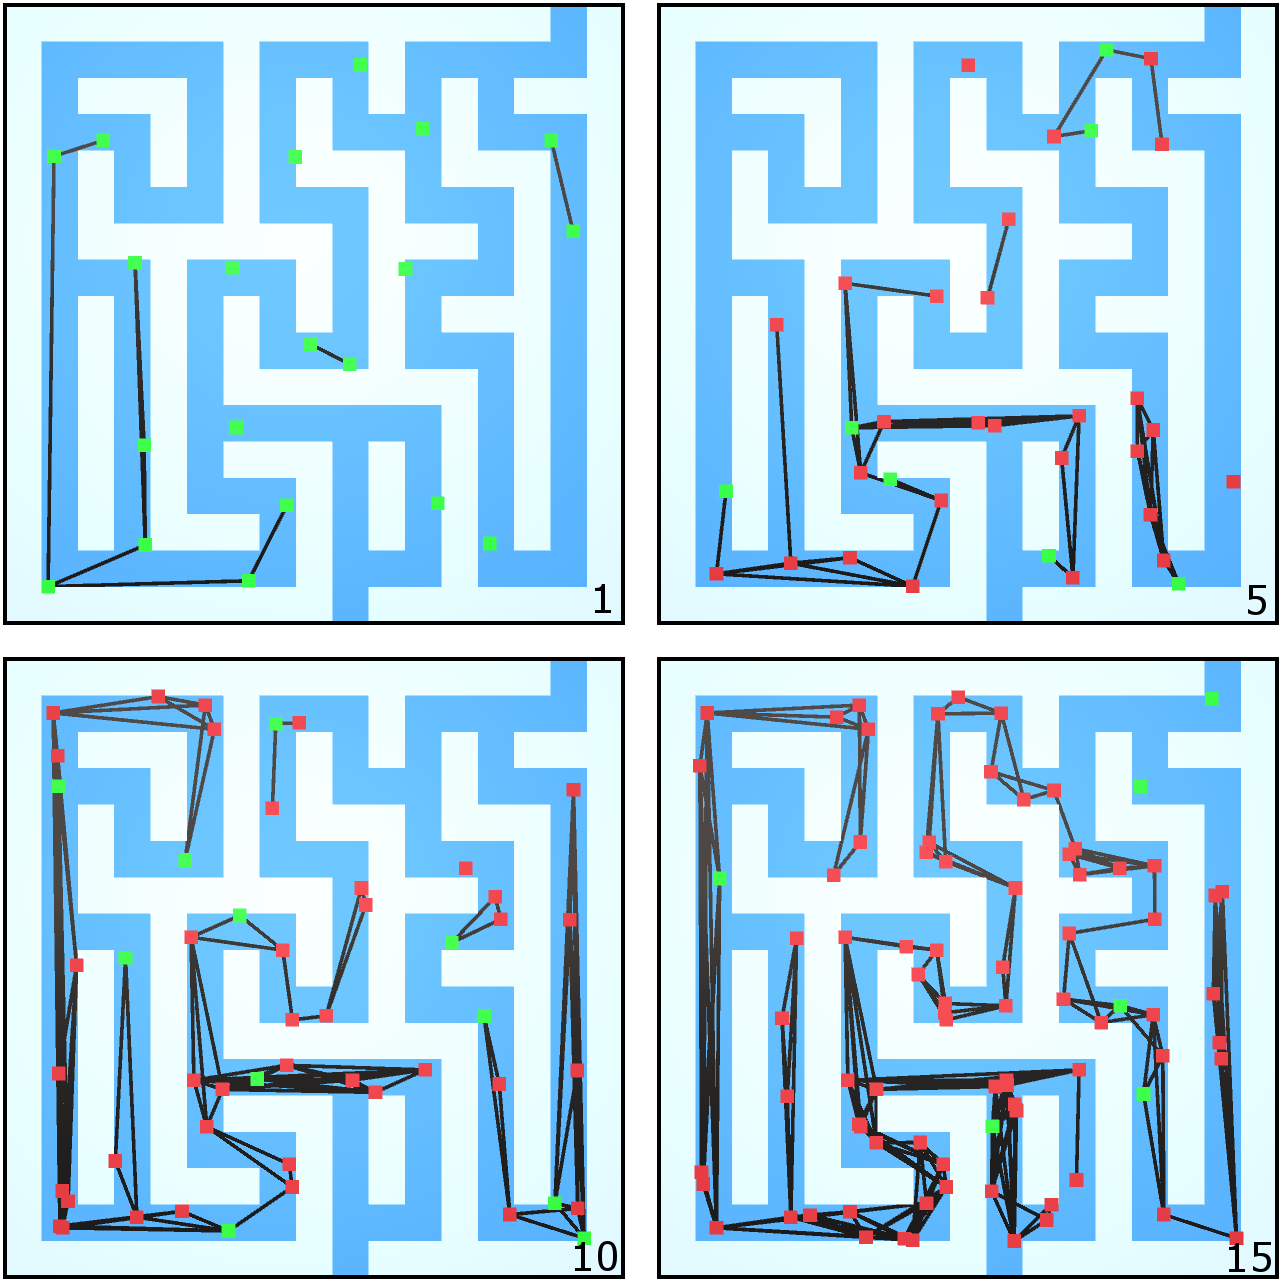
\includegraphics[width=1\columnwidth]{tests/geneticT3b}
		\caption{The most fit waypoint graphs from the 3rd trial of our genetic algorithm. Sampled at generations 1, 5, 10, and 15 respectively. Red nodes are inherited from previous generations, while freshly created nodes are labeled in green.}
	\end{figure}
	
	\begin{figure*}
		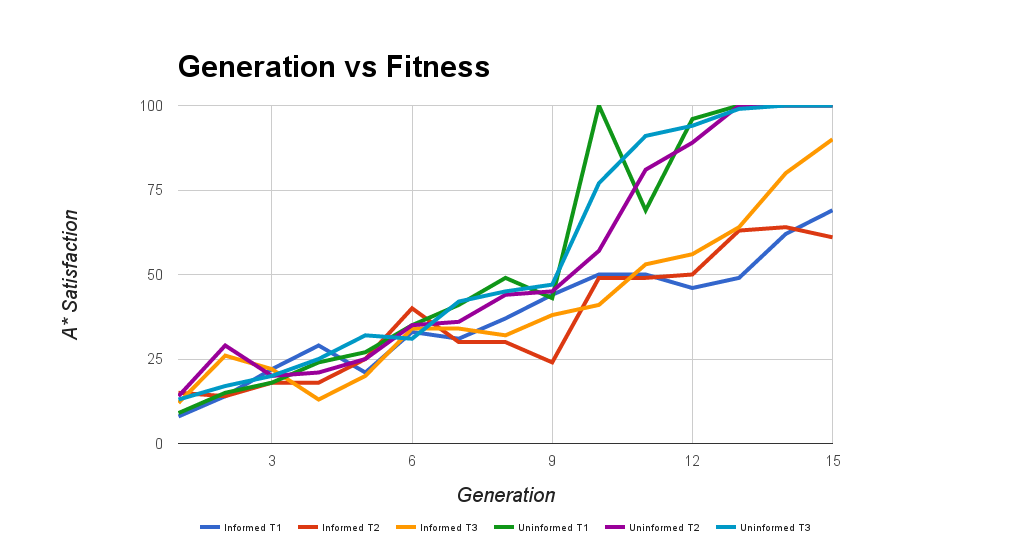
\includegraphics[width=\textwidth]{tests/genfitness}
		\caption{Red, Blue and Orange show the trials using our genetic algorithm, while Green, Purple and Cyan show trials using uninformed node placement.}
	\end{figure*}
	
	\begin{figure*}
		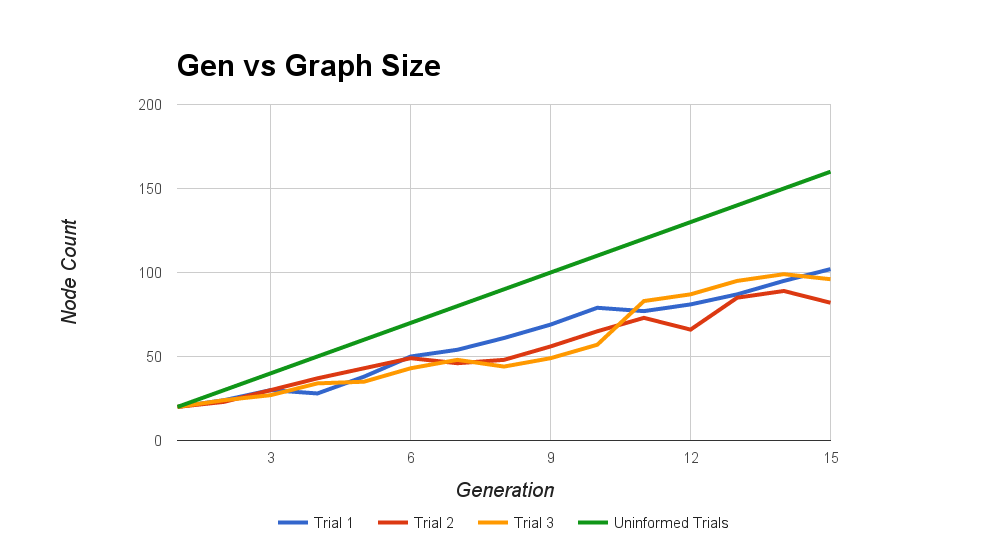
\includegraphics[width=\textwidth]{tests/gengraphsize}
		\caption{Green shows graph size growth for uninformed trials, while Red, Green and Orange show graph size for trials using our genetic algorithm. The uninformed system uses significantly more nodes, which is undesirable for A*.}
	\end{figure*}
	
	\begin{figure*}
		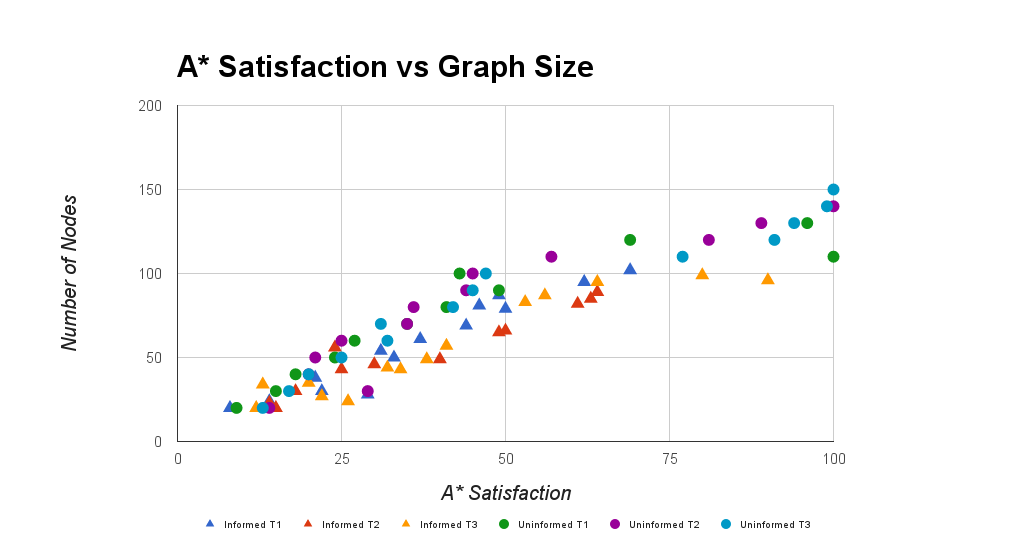
\includegraphics[width=\textwidth]{tests/satgraphsize}
		\caption{The Genetic algorithm (Triangles) consistently demonstrates that it requires far fewer nodes than the uninformed system to achieve approximately the same A* Satisfaction rating. (Circles)}
	\end{figure*}
	
	\subsection{Algorithm Refinement}
	Over the course of our development we experimented with multiple different maze configurations, constraint tuning, and crossover adjustments. Early on in development, a larger graph was used to demonstrate the basic functionality of the various genetic algorithm components. However, once the full algorithm was implemented, we chose to instead opt for a significantly smaller graph, which significantly improved runtime usability and allowed for a much easier comparison between graphs within the same population as well as comparisons from generation to generation. The smaller graph also allowed the initial population to begin with a fitness of 10-20\% A* satisfaction, up from 1\% with the large maze, which helped reduce the number of nodes required to start a generation, thus allowing the algorithm to run a little quicker.
	
	\subsubsection{Crossover Refinements}
	Many of the improvements that were made were also related to the crossover stage of the algorithm. Specifically, there were several major changes that were made to improve generational A* satisfaction progress, as well as reduce the number of nodes required to reach higher satisfaction values.
	
	Initially, crossover was implemented simply as a breeding stage, merging half of the nodes from each parent into a child graph. As the algorithm began to take shape however, it was quickly discovered that overly homogeneous populations were causing the graphs to decline in fitness from generation to generation. To rectify this issue, we modified the crossover stage to instead cycle out about 10\% of the nodes from the parents and instead replace them with new nodes.
	
	Additionally, we recognized that the graph size would need to fluctuate in order to properly cover the maze's walkable area and improve fitness. Initially we had the graphs grow at a predictable steady rate at each generation, however after testing this system, we found that high A* satisfaction was likely only being reached by over saturating the maze with nodes. Our alternative approach involved modifying how many nodes would replace the 10\% that were originally removed. In order to prevent the graphs from growing indefinitely, we implemented a system to grow the graph depending on it's parent's A* satisfaction rating. The higher a parent's A* satisfaction rating, the fewer nodes will be added to it's children. This also allows the node count to plateau after a certain number of generations, and in some cases decrease after a certain point.
	
	
	
	
	
	